\chapter{Gestión del proyecto}

% **************************** Define Graphics Path **************************
\ifpdf
    \graphicspath{{Chapter7/Figs/Raster/}{Chapter7/Figs/PDF/}{Chapter7/Figs/}}
\else
    \graphicspath{{Chapter7/Figs/Vector/}{Chapter7/Figs/}}
\fi

En el presente cap\'itulo se realiza un breve análisis acerca de la ejecuci\'on del proyecto, mostrando de las principales actividades y lineas de trabajo seguidas, las respectivas fechas de inicio y fin de las actividades, destacando en los casos en que corresponde las posibles dependencias y atrasos.

\section{Ejecuci\'on del proyecto}

En la figura \ref{fig:gantt} se muestra un diagrama de Gantt con las actividades m\'as importantes durante la ejecuci\'on de este proyecto, con sus respectivas fechas de inicio y fin.

\begin{figure}[h!] 
\centering    
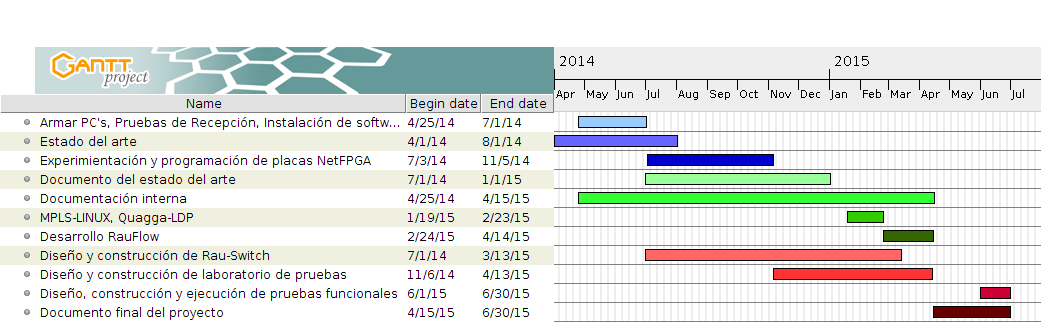
\includegraphics[width=1.00\textwidth]{ganttDP}
\caption[Diagrama de Gantt, Actividades del Proyecto]{Diagrama de Gantt, Actividades del Proyecto}
\label{fig:gantt}
\end{figure}

A continuaci\'on se describen los principales contratiempos experimentados en la ejecuci\'on de cada una de estas actividades.

\textbf{Armar PC's, Pruebas de Recepción, Instalación de sotware b\'asico:} Esta linea de trabajo engloba las actividades realizadas al inicio del proyecto en las que se monta la plataforma base de cuatro dispositivos RAU-Switch utilizados adem\'as como estaci\'on de trabajo durante toda la ejecuci\'on del proyecto. En esta etapa se recibe el hardware utilizado (PC's, tarjetas NetFPGA, transceiver SFP y patch cords de fibra entre otros), se realiza un inventario, pruebas de aceptaci\'on y se procede con la instalaci\'on del hardware y software b\'asico (Sistema Operativo, suite de desarrollo de Xlinix entre otros).\\

Dentro de esta etapa son cr\'iticas la recepci\'on de todos los dispositivos de hardware y las pruebas de recepci\'on. Cabe destacar sobre esto, el 14/04/2014 se reciben las primeras dos PC's con las cuales empezar a trabajar, y [no encontramos la fecha] llegan las cinco placas NetFPGA.\\

\textbf{Estado del Arte} Esta linea de trabajo se desarrolla sin contratiempos aunque se extiende un mes m\'as de lo previsto cuando comienza la etapa de experimientaci\'on con el hardware.\\ 
  
\textbf{Experimentaci\'on y programaci\'on de las placas NetFPGA} Esta linea de trabajo engloba actividades como la programaci\'on del hardware con los diferentes proyectos disponibles (de referencia y comunitarios), aprendizaje del entorno de desarrollo, evaluar la posibilidad de programar directamente el hardware con desarrollos propios, diseñar una estrategia de implementaci\'on para RAU-Switch.\\

Dentro de esta etapa es critica la obtenci\'on de un paquete de licencias pagas especiales para la suite de Xilinx ISE SDK. Oficialmente se obtiene este paquete el 29/10/2014 aunque el 16/10/2014 se obtiene una soluci\'on provisoria a este problema. A su vez es critico de esta etapa completar la programaci\'on persistente del hardware sin errores en el funcionamiento, hecho que sucede el día 05/11/2014.\\

\textbf{Documento del estado del Arte:} Esta actividad se realiza en paralelo con el resto de las actividades del proyecto, teniendo dos iteraciones para la generación de un documento del estado del arte previo al expuesto en el informe final del proyecto. Estas son el 15/09/2014 y el 01/12/2015.\\

\textbf{Documentacion interna:} Esta actividad se desarrolla en el transcurso de todo el proyecto orientada a la redacci\'on del documento final del proyecto.

\textbf{MPLS-Linux, Quagga-LDP:} Esta linea de trabajo engloba las actividades de experimentaci\'on realizada con ambas herramientas durante la fase de construcci\'on de RAU-Switch. A pesar del tiempo invertido en esta actividad no se obtienen los resultados esperados y se decide abandonar esta linea de trabajo sopesando el tiempo invertido.\\

Esta actividad es critica en el desarrollo de RAUFlow no permitiendo comenzar con esta \'ultima hasta que se finalizara.\\

\textbf{Desarrollo de RAUFlow:} Esta linea de trabajo engloba las actividades de diseño e implementaci\'on de RAUFlow. Se invierte poco m\'as de un mes en esta actividad debido al atraso general en el cronograma del proyecto, sacrificando un conjunto bastante interesante de funcionalidades de la aplicaci\'on.

\textbf{Diseño y construcci\'on de RAU-Switch:} Esta linea de trabajo engloba actividades de progrmaci\'on, experimentaci\'on e investigaci\'on con diferentes herramientas de software y el hardware utilizado, hasta alcanzar la construcci\'on del dispositivo en cuesti\'on. Como etapa en el proyecto comienza una vez que se finalizan las pruebas de recepci\'on de hardware, y finaliza una vez que se alcanza un producto estable funcionalmente.\\

Como etapa de proyecto son criticas las pruebas de recepci\'on de hardware, las cuales habilitan una vez concluidas comenzar a trabajar en la misma.\\

\textbf{Diseño y construcci\'on del laboratorio de pruebas:} Comienza como etapa cuando culmina la etapa de experimentaci\'on con el hardware y comienza a pensarse en el diseño de RAU-Switch y de un laboratorio de pruebas utilizando los cuatro nodos disponibles, y culmina el 13/04/2015 cuando se reciben las \'ultimas componentes de hardware necesarias para la construcci\'on del mismo.\\

\textbf{Diseño, implementaci\'on y ejecuci\'on de pruebas funcionales:} Engloba todas las actividades de verificaci\'on del prototipo construido utilizando el laboratorio de pruebas.\\

Son criticas para realizar las actividades de ejecuci\'on de pruebas el contar con el laboratorio de pruebas construido y una versi\'on estable de RAUFlow.\\

\textbf{Documentaci\'on del proyecto:} Si bien a lo largo de todo el proyecto se genera documentaci\'on  , es de carácter interno. La elaboraci\'on del documento final de proyecto se posterga hasta el momento de contar con una versi\'on estable de RAUFlow, lo cual sucede el 15/04/15.